\documentclass{standalone}
\usepackage{tikz}
\usetikzlibrary{shapes}
\begin{document}
    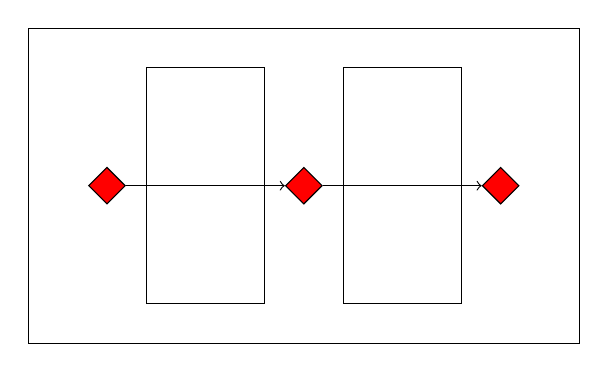
\begin{tikzpicture}
       \draw (0,-0.5) rectangle (7,3.5);
       \node[draw, diamond,fill=red] (m1) at (1,1.5) {};
       \draw (1.5,0) rectangle (3,3);
       \node[draw, diamond,fill=red] (m2) at (3.5,1.5) {};
       \draw (4,0) rectangle (5.5,3);
       \node[draw, diamond,fill=red] (m3) at (6,1.5) {};
       \draw[->] (m1) -- (m2);
       \draw[->] (m2) -- (m3);
    \end{tikzpicture}
\end{document}